\documentclass[xetex,mathserif,serif]{beamer}
\usepackage{polyglossia}
\setdefaultlanguage[babelshorthands=true]{russian}
\usepackage{minted}
\usepackage{tabu}
\usepackage{graphicx}

\usepackage{adjustbox}

\useoutertheme{infolines}

\usepackage{fontspec}
\setmainfont{FreeSans}
\newfontfamily{\russianfonttt}{FreeSans}

\definecolor{links}{HTML}{2A1B81}
\hypersetup{colorlinks,linkcolor=,urlcolor=links}

\setbeamertemplate{blocks}[rounded][shadow=false]
\setbeamercolor*{block title alerted}{fg=red!50!black,bg=red!20}
\setbeamercolor*{block body alerted}{fg=black,bg=red!10}

\tabulinesep=0.8mm

\title{Автоматическая типизация горных пород}
\author{Александр Смирнов}
\date{27.12.2019г}

\begin{document}


	\frame{\titlepage}


	\begin{frame}
		\frametitle{Введение}
		
		\begin{itemize}
	    	\item Способ разведки нефтяных месторождений — разведка буром
        	    \begin{itemize}
        	    	\item Во время бурения извлекают керн
        	    	\item Видно, как залегают пласты породы
        	    	\item Позволяют обнаружить породы-коллекторы, оценить их емкостные и фильтрационные свойства
            	\end{itemize}
            \item Керн — цилиндрический монолит горной породы, получаемый путём кольцевого разрушения забоя скважин при бурении
        \end{itemize}	
        
        \begin{figure}[h]
            \label{керн}
            \centering
            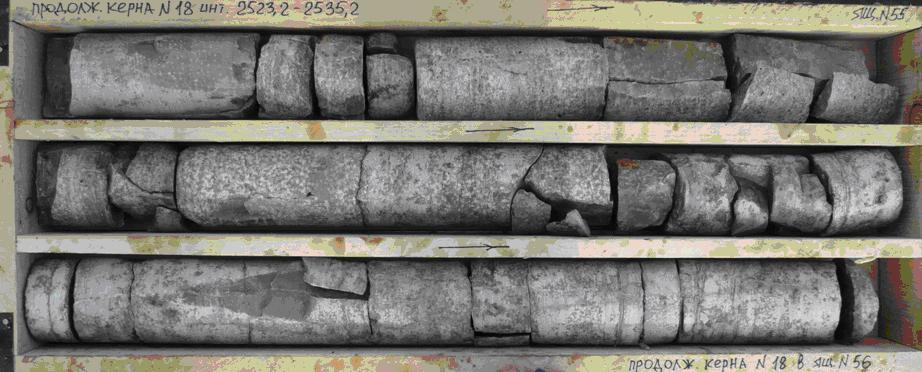
\includegraphics[scale=0.25]{images/kern.jpg}
            \caption{Пример керна}
        \end{figure}
        
	\end{frame}


	\begin{frame}
		\frametitle{Введение (2)}
		
		\begin{itemize}
	    	\item Фотографии керна в ультрафиолетовом свете
        	    \begin{itemize}
        	    	\item Позволяют выделить в разрезе нефтенасыщенные участки
        	    	\item Позволяют выделить текстурные характеристики, связанные с особенностями условий осадконакопления пород
            	\end{itemize}
        \end{itemize}	
        
        \begin{figure}[h]
            \centering
            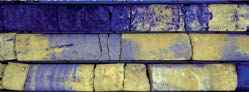
\includegraphics[scale=0.6]{images/UV.png}
            \caption{Фотографии керна в ультрафиолетовом свете. Неравномерное желтое свечение – неравномерно нефтенасыщенный песчаник.}
            \label{UV}
        \end{figure}   
        
	\end{frame}	
	
	
	\begin{frame}
		\frametitle{Проблема}
		
		\begin{itemize}
	    	\item Информация о керне описывается послойно: один слой - один тип породы
	    	\item Можно размечать изображения керна с большей точностью 
    		\begin{itemize}
    	    	\item Более точные модели пластов
            \end{itemize} 	    	
        \end{itemize} 
        
	\end{frame}		
	
	
	\begin{frame}
		\frametitle{Цели}
		
		\begin{itemize}
	    	\item Получение описания керна на основе выборки фотографий
    		\begin{itemize}
                \item Тип породы с точностью до 20 см. 
                \item Карбонатность с точностью до 10 см.
                \item Нефтенасыщенность с точностью до 10 см.
                \item Разрушенность с точностью до 5 см.
            \end{itemize}
            \item Написание удобной для пользователя обёртки над полученным решением для последующего использования   	
        \end{itemize} 
        
	\end{frame}		
	
	
	\begin{frame}
		\frametitle{Задачи}
		
        \begin{itemize}
            \item Произвести разведочный анализ предоставленных данных
            \item Ознакомиться с возможными решениями
            \item Реализовать решения и найти лучшие
            \item Сравнить результаты с уже имеющимися у заказчика
            \item Создать оболочку для удобного использования решения
        \end{itemize} 
        
	\end{frame}		
	
	
	\begin{frame}
		\frametitle{Исходные данные}

        \begin{itemize}
            \item Фотографии керна
            \item Те же самые фотографии керна, но в ультрафиолетовом освещении
        \end{itemize} 
    
        \begin{figure}[h]
            \centering
            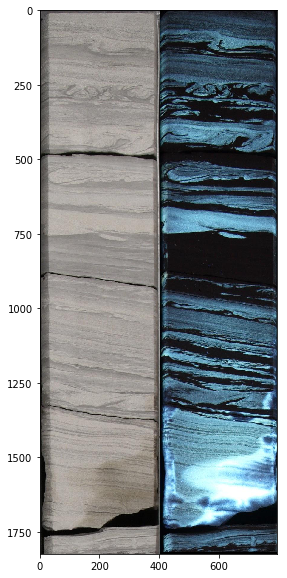
\includegraphics[scale=0.2]{images/sample.png}
            \caption{Пример из исходных данных. Слева — фото керна, справа — фото того же керна, но в УФ.}
            \label{sample}
        \end{figure}       
    
	\end{frame}		
	
	
	\begin{frame}
		\frametitle{Исходные данные (2)}

        \begin{itemize}
            \item Таблица с описанием каждой фотографии
            \item Необходимо предсказывать:
            \begin{itemize}
                \item Rock (тип породы)
                \item Carbonate (карбонатность)
                \item Ruin (разрушенность)
                \item Saturation (нефтенасыщенность)
            \end{itemize}
        \end{itemize} 

        \begin{table}[]
            \centering
            \begin{adjustbox}{width=150,center}
            \begin{tabular}{|l|l|l|}
                \hline
                {} &                0 &                1 \\
                \hline
                Id             &          1000000 &          1000001 \\
                PhotoTop       &                0 &                0 \\
                PhotoDown      &                1 &                1 \\
                Rock           &         песчаник &         песчаник \\
                Carbonate      &   не карбонатный &   не карбонатный \\
                Ruin           &      не разрушен &      не разрушен \\
                Saturation     &  нефтенасыщенные &  нефтенасыщенные \\
                \hline
            \end{tabular}
            \end{adjustbox}
            \caption{Пример из таблицы исходных данных. Предоставлена информация о первых двух записях — один и тот же керн, обычная фотография и фотография в УФ.}
            \label{sample_table_cleaned} 
        \end{table}      
        
	\end{frame}		
	
	
	\begin{frame}
		\frametitle{Анализ данных}

        \begin{itemize}
            \item Поля \textbf{PhotoUp} и \textbf{PhotoDown} означают начало и конец данной фотографии в данном образце керна
            \item \textbf{PhotoUp}=0 и \textbf{PhotoDown}=1 $\Rightarrow$ длина керна на фотографии — 1 метр
            \item В категории \textbf{Rock} очень много значений, которые имеют малое количество экземпляров в сравнении с другими категориями $\Rightarrow$ выбросим их после согласования с заказчиком
        \end{itemize} 
    
        \begin{table}[]
            \centering
            \begin{tabular}{|l|c|}
                \hline
                \textbf{тип породы} & \textbf{количество экземпляров} \\
                \hline
                песчаник            & 2482                            \\
                \hline
                аргиллит            & 1220                            \\
                \hline
                алевролит           & 1138                            \\
                \hline
                переслой            & 686                            \\
                \hline
            \end{tabular}
            \caption{Распределение категории "тип породы".}
            \label{table_rock}  
        \end{table}    
    
	\end{frame}	
	
	
	\begin{frame}
		\frametitle{Анализ подходов}
		
        \begin{itemize}
            \item Классификация изображений 
            \item Распознавание образов на изображениях
            \item Сегментация изображений
        \end{itemize} 
        
	\end{frame}	
	
	
	\begin{frame}
		\frametitle{Анализ подходов (2)}
		
        \begin{itemize}
            \item Задача классификации — определяем входное изображение в один из классов
            \item Методы машинного обучения
                \begin{itemize}
                    \item Выделяем признаки с помощью алгоритмов
                        \begin{itemize}
                            \item Гистограмма направленных градиентов
                            \item Метод Виолы — Джонса
                        \end{itemize}
                    \item Используем техники классификации
                        \begin{itemize}
                            \item SVM
                        \end{itemize}
                \end{itemize} 
            \item Методы глубокого обучения
                \begin{itemize}
                    \item Свёрточные нейронные сети
                \end{itemize}
            \item Лучшие решения — свёрточные нейронные сети
        \end{itemize} 
        
	\end{frame}		


	\begin{frame}
		\frametitle{Анализ подходов (3)}
		
        \begin{itemize}
            \item Задача распознавания образов — определяем на фотографии границы объектов известных классов
            \item То же, что и классификация, только с помощью алгоритмов сужаем область, в которой находится объект
            \item Для более точного распознавания подаём на вход не только фотографию с отмеченной категорией, но и область, в которой находится данный объект
        \end{itemize} 
        
	\end{frame}	
	
	
	\begin{frame}
		\frametitle{Анализ подходов (4)}
		
        \begin{itemize}
            \item Сегментация изображений — это процесс присвоения таких меток каждому пикселю изображения, что пиксели с одинаковыми метками имеют общие визуальные характеристики
            \item Для достижения большей точности некоторые алгоритмы помимо фотографии принимают изображение с размеченными по категориям пикселями
        \end{itemize} 
        
        \begin{figure}[h]
            \centering
            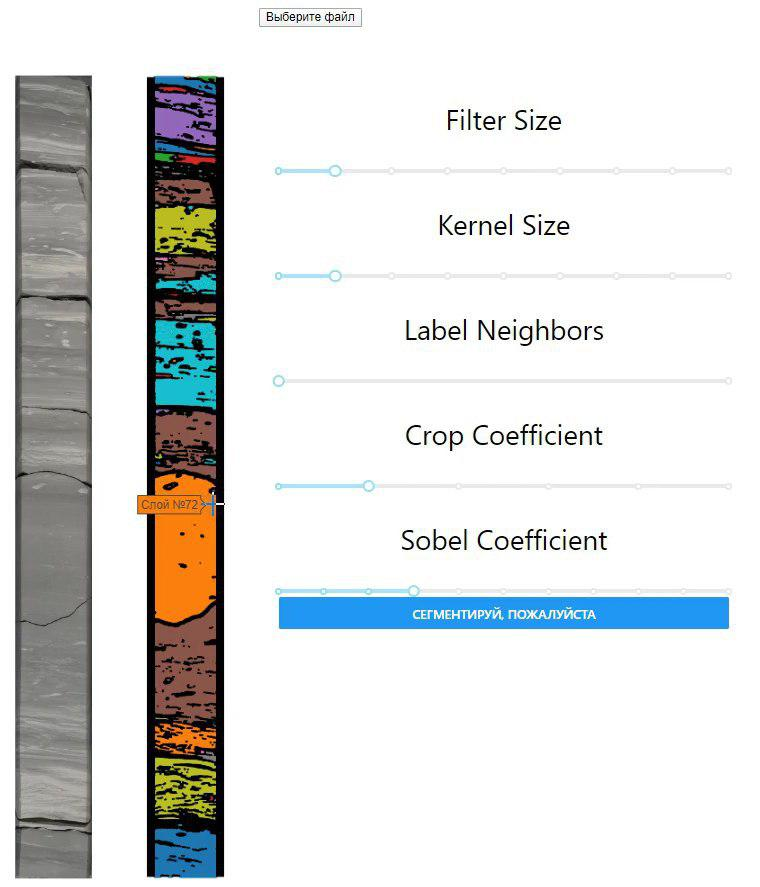
\includegraphics[scale=0.15]{images/segmentation.jpg}
            \caption{Пример работы сегментационного алгоритма.}
            \label{segmentation}
        \end{figure}        
        
	\end{frame}		


	\begin{frame}
		\frametitle{Решение}
		
        \begin{itemize}
            \item Будем решать задачу классификации
            \item Подготовим данные
            \item Выберем алгоритм
            \item Сравним результаты
        \end{itemize} 
        
	\end{frame}	


	\begin{frame}
		\frametitle{Подготовка данных}
		
        \begin{itemize}
            \item В каждой категории классификации количество экземпляров не сбалансировано $\Rightarrow$ применяем \textbf{oversampling} (увеличение количества экземпляров в недостающих классах путём их копирования)
                \begin{itemize}
                    \item Алгоритмы не учитывают перевес одних классов над другими в количестве элементов
                \end{itemize}
            \item Категории должны быть определены с фиксированной точностью $\Rightarrow$ на вход поступает фотография керна высотой, к примеру, 1 метр, она разделяется на 5 фотографий керна длиной 20 сантиметров каждая
            \item Подготовленные подобным образом фотографии будут подаваться на вход ниже описанным алгоритмам
        \end{itemize} 
        
	\end{frame}	

        
	\begin{frame}
		\frametitle{Выбор алгоритмов}
		
        \begin{itemize}
            \item Свёрточная нейронная сеть.
            \item Feature extraction на основе свёрточной нейронной сети + kNN
        \end{itemize} 
        
	\end{frame}	
	
	
	\begin{frame}
		\frametitle{Свёрточная нейронная сеть}
		
        \begin{itemize}
            \item Имеются данные двух типов — обычные фотографии и фотографии в ультрафиолетовом свете
            \item Будем использовать предобученные модели
            \item Возможные решения:
                \begin{itemize}
                    \item Отдельно обучать алгоритмы на классификацию обычных фотографий и фотографий в УФ. Объединять их выводы.
                    \item Имея в сумме 6 каналов цвета из двух трёхканальных фотографий, можно обучать алгоритмы выборочно по 3-м каналам
                    \item Обучать $C_{6}^{3}=20$ алгоритмов на каждую тройку каналов. Объединять их выводы
                \end{itemize}
        \end{itemize} 
        
	\end{frame}	
	
	
	\begin{frame}
		\frametitle{Свёрточная нейронная сеть (2)}
		
        \begin{itemize}
            \item Рассмотрим первый подход
            \item Протестируем и сравним точность предобученных архитектур
            \item Преобразуем наши изображения до формата входных данных обученных сетей
        \end{itemize} 
        
        \begin{table}[h!]
            \centering
            \begin{tabular}{|c|c|c|c|c|}
            \hline
            \textbf{data type} & \textbf{model} & \textbf{epochs} & \textbf{val acc} & \textbf{roc auc} \\ \hline
            non-UV             & VGG16          & 3               & 0.75             & \textbf{0.93}    \\ \hline
            non-UV             & ResNet50       & 60              & 0.69             & 0.85             \\ \hline
            non-UV             & DenseNet121    & 221             & 0.6              & 0.7              \\ \hline
            non-UV             & Xception       & 34              & 0.62             & 0.74             \\ \hline
            UV                 & VGG16          & 11              & 0.72             & \textbf{0.88}    \\ \hline
            UV                 & ResNet50       & 71              & 0.62             & 0.77             \\ \hline
            UV                 & DenseNet121    & 154             & 0.52             & 0.64             \\ \hline
            UV                 & Xception       & 60              & 0.49             & 0.55             \\ \hline
            \end{tabular}
            \caption{Результаты использования предобученных архитектур на примере классификации типа породы.}
            \label{results}   
        \end{table}        
        
	\end{frame}	
	
	
	\begin{frame}
		\frametitle{Свёрточная нейронная сеть (3)}
		
        \begin{itemize}
            \item Top-1 accuracy вышла 0.75
            \item Неплохо, учитывая, что мы используем только половину информации
            \item Данный подход может дать ещё большую точность, если эту модель совместить с моделью для классификации по УФ фотографиям
        \end{itemize}    
        
	\end{frame}	
	
	
	\begin{frame}
		\frametitle{Заключение}
		
        \begin{itemize}
            \item Что было сделано в рамках данной работы
                \begin{itemize}
                    \item Изучена предметная область
                    \item Провёдены изучение и подготовка данных
                    \item Провёден разбор возможных решений
                    \item Реализовано одно решение 
                \end{itemize}
            \item Что планируется сделать
                \begin{itemize}
                    \item Улучшить реализованное решение
                    \item Реализовать метрическую классификацию
                    \item Реализовать распознавание и сегментацию
                    \item Сравнить результаты между собой
                    \item Обернуть решение в удобный интерфейс
                \end{itemize}  
        \end{itemize}    
        
	\end{frame}		
	 

\end{document}